\documentclass[master]{ntuthesis}

\usepackage{fancyhdr}              % Extensive control of page headers and footers
\usepackage[normalem]{ulem}        % Package for underlining
\usepackage[hyphens]{url}          % URL wrapper with break on hypthens
\usepackage{pdfpages}              % PDF page inseration
%\usepackage[sort,nocompress]{cite} % Sort the citations
\usepackage[toc,page]{appendix}    % Extra control of appendices
% Always include hyperref last
\usepackage[colorlinks=false,unicode]{hyperref} % Generating bookmarks and links in PDF file

% Solving the bug of conflict in xeCJK with listing (should be fixed in the near future)
% https://github.com/CTeX-org/ctex-kit/issues/297
\ifxetex
\ExplSyntaxOn
\bool_new:N \l__xeCJK_listings_letter_bool
\ExplSyntaxOff
\fi
% End of solving bugs

% My packages
% READMORE
% https://tex.stackexchange.com/questions/12672/which-tabular-packages-do-which-tasks-and-which-packages-conflict
\usepackage{caption}    % captionof for assigning subfigure in minipage
\usepackage{graphics}   % includegraphics
\usepackage{subfigure}  % for figure
\usepackage{tabularx}   % Provides a column type which expands to fill the specified width of the table
\usepackage{array}      % offers more flexible column formatting; fixes to some spacing issues
\usepackage{tabulary}   % Provides column types which are proportional to the natural width of their contents
\usepackage{multirow}   % Lets tabular material span multiple rows
\usepackage{booktabs}   % Supports professional looking tables; better vertical spacing; better rules
\usepackage{makecell}   % Multiple line cells, better headers, thick lines, diagonally divided cells, etc.
\newcolumntype{K}[1]{>{\centering\arraybackslash}m{#1}} % Convenient column type

% These are all for programing languages
\usepackage{algorithm, algorithmicx, algpseudocode} % Pseudo Code
\usepackage{minted}     % Using external tools for rendering codes
\usepackage{listings}   % listing is an alternative solution for colored codes
\usepackage{color}      % color macros

\definecolor{dkgreen}{rgb}{0,0.6,0}
\definecolor{gray}{rgb}{0.5,0.5,0.5}
\definecolor{mauve}{rgb}{0.58,0,0.82}

\lstset{frame=tb,
  language=C++,
  aboveskip=3mm,
  belowskip=3mm,
  showstringspaces=false,
  columns=flexible,
  basicstyle={\small\ttfamily},
  numbers=none,
  numberstyle=\tiny\color{gray},
  keywordstyle=\color{blue},
  commentstyle=\color{dkgreen},
  stringstyle=\color{mauve},
  breaklines=true,
  breakatwhitespace=true,
  tabsize=3
}
% End of my packages

% Your information goes here
% author: Medicine Yeh
% origin: Tz-Huan Huang [http://www.csie.ntu.edu.tw/~tzhuan]

% ----------------------------------------------------------------------------
% "THE CHOCOLATE-WARE LICENSE":
% Tz-Huan Huang wrote this file. As long as you retain this notice you
% can do whatever you want with this stuff. If we meet some day, and you think
% this stuff is worth it, you can buy me a chocolate in return Tz-Huan Huang
% ----------------------------------------------------------------------------

% Syntax: \var{English}{Chinese}
\university{National Taiwan University}{國立臺灣大學}
\college{College of Electrical Engineering and Computer Science}{電機資訊學院}
\institute{Department of Computer Science and Information Engineering}{資訊工程學系}
\title{The TITLE}{標題在這}
\author{ABC Ming}{王小民}
\studentid{R01234567}
\advisor{ABC Ming, Ph.D.}{王大民~博士}
\defenseyear{2017}{106}
\defensemonth{June}{6}
\defenseday{12}
\doi{doi:10.6342/NTU2017XXXXX}
\keywords{
keyword1, keyword2
}{
關鍵字1、關鍵字2
}


% Force use other fonts (Un-comment this line and set to the right font family you have)
%
%\setmainfont{Times New Roman}
%\setCJKmainfont{標楷體}
%\setmainfont{Liberation Serif} % Free English Font
%\setCJKmainfont{Kaiti TC}  % Apple MAC OS
%\setCJKmainfont[BoldFont={cwTeXHeiBold}]{cwTeXKai} % Free CJK Font



% Useful command samples provided by this template
%\removedoi        % Remove doi after this page (included)
%\removewatermark  % Remove watermark after this page (included)

\begin{document}

\insertdoi         % Insert doi after this page (included)
\insertwatermark   % Insert watermark after this page (included)

\frontmatter
    \maketitlepage
    %-----------           reset numbering system         -----------
    \pagenumbering{roman}  % Reset number format
    \setcounter{page}{1}   % Reset page number
    %----------- generate/include the certification page  -----------
    \makecertification[angle=0]{certification.pdf}  % angle=180 for up-side-down image
    \begin{acknowledgementszh}
感謝Tz\-Huan Huang提供了初版Xe\LaTeX{}板型,基於該程式碼,本專案提供更完整且多功能的模板。
另外此模板也提供範例程式碼讓初寫論文的人可以快速上手\LaTeX{}。
%
\end{acknowledgementszh}

%\begin{acknowledgementsen}
% English version of acknowledgements is not required by NTU.
%
%\end{acknowledgementsen}

    \begin{abstractzh}
本論文提出了一影像中使用者感興趣區域 (region of interest)
偵測之資料集 (benchmark)。
使用者感興趣區域偵測在許多應用中極為有用,
過去雖然有許多使用者感興趣區域之自動偵測演算法被提出,
然而由於缺乏公開資料集,
這些方法往往只測試了各自的小量資料而難以互相比較。
從其它領域可以發現,
基於公開資料集的可重製實驗與該領域突飛猛進密切相關,
因此本論文填補了此領域之不足,
我們提出名為「Photoshoot」的遊戲來蒐集人們對於感興趣區域的標記,
並以這些標記來建立資料集。
透過這個遊戲,我們已蒐集大量使用者對於感興趣區域的標記,
並結合這些資料成為使用者感興趣區域模型。
我們利用這些模型來量化評估五個使用者感興趣區域偵測演算法,
此資料集也可更進一步作為基於學習理論演算法的測試資料,
因此使基於學習理論的偵測演算法成為可能。

\end{abstractzh}

\begin{abstracten}
This thesis presents a benchmark for region of interest (ROI)
detection. ROI detection has many useful applications and many
algorithms have been proposed to automatically detect ROIs.
Unfortunately, due to the lack of benchmarks, these methods were
often tested on small data sets that are not available to others,
making fair comparisons of these methods difficult. Examples from
many fields have shown that repeatable experiments using published
benchmarks are crucial to the fast advancement of the fields. To
fill the gap, this thesis presents our design for a collaborative
game, called Photoshoot, to collect human ROI annotations for
constructing an ROI benchmark. With this game, we have gathered a
large number of annotations and fused them into aggregated ROI
models. We use these models to evaluate five ROI detection
algorithms quantitatively. Furthermore, by using the benchmark as
training data, learning-based ROI detection algorithms become
viable.

\end{abstracten}

\begin{comment}
\category{I2.10}{Computing Methodologies}{Artificial Intelligence --
Vision and Scene Understanding} \category{H5.3}{Information
Systems}{Information Interfaces and Presentation (HCI) -- Web-based
Interaction.}

\terms{Design, Human factors, Performance.}

\keywords{Region of interest, Visual attention model, Web-based
games, Benchmarks.}
\end{comment}

    %-----------        Generate lists and indices        -----------
    \tableofcontents
    \listoffigures
    \listoftables

\mainmatter
    % Your thesis goes here
    \chapter{Introduction}
\label{c:intro}

Attention plays an important role in human vision. For example, when
we look at an image, our eye movements comprise a succession of {\em
fixations} (repetitive positioning of eyes to parts of the image)
and {\em saccades} (rapid eye jump). Those parts of the image that
cause eye fixations and capture primary attention are called {\em
regions of interest} (ROIs). Studies in visual attention and eye
movement have shown that humans generally only attend to a few ROIs.
Detecting these visually attentive regions in images is challenging
but useful in many multimedia applications, such as automatic
thumbnail cropping, object recognition, content-based image
retrieval, adaptive image compression and automatic browsing in
small-screen devices.

Many algorithms have been proposed for automatic ROI detection in
images. Unfortunately, these methods were often evaluated only on
specific and small data sets that are not publicly available. The
lack of published {\em benchmarks} makes experiments non-repeatable
and quantitative evaluation difficult. However, as recommended by
the latest ACM SIGMM retreat, repeatable experiments using published
benchmarks are important for advancing the multimedia research
field~\cite{Rowe:2005:ASR,intel_ocl_spm}, Figure~\ref{kl}.

\begin{figure}
\centering
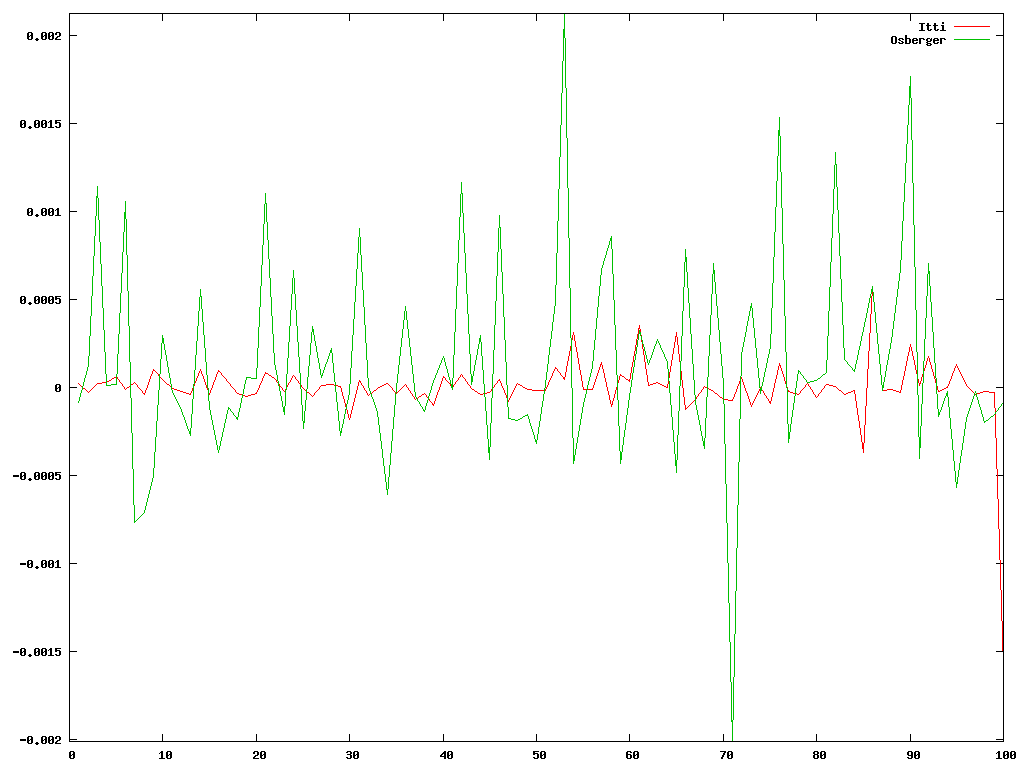
\includegraphics[width=0.45\textwidth]{figures/kl}
\caption{kl-distance}
\label{kl}
\end{figure}

\begin{table}[t]
\begin{center}
\begin{tabular}{lcc}

\hline
                    &  {\small Itti's method}     & {\small Fuzzy growing}    \\
\hline
{\small Precision}           &  0.4475    & 0.4506 \\
{\small Recall}              &  0.5515    & 0.5542 \\
\hline

\end{tabular}
\caption[Evaluation of FOA sets]{\small Evaluation of FOA sets. } \label{t:FOA}
\end{center}
\end{table}

    \chapter{Background and Relatedwork}
\label{chap:relatedworks}

    \chapter{Implementation}
\label{chap:implementation}

    \chapter{Evaluations}
\label{chap:evaluations}

    \chapter{Introduction}
\label{chap:conclusion}

    \appendix

\backmatter
    \makebibliography
    \bibliographystyle{abbrv}
    % Your bibliography goes here
    \bibliography{thesis}

\end{document}
